\documentclass[12pt,a4paper]{article}
\usepackage[utf8]{inputenc}
\usepackage[french,english]{babel}
\usepackage{graphicx}
\usepackage{geometry}
\geometry{margin=2.5cm}
\usepackage{setspace}
\setlength{\parskip}{0.5em}

\begin{document}
\thispagestyle{empty}

%-------------------------
% Header with logos
%-------------------------
\begin{minipage}{0.2\linewidth}
  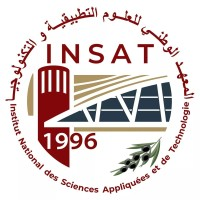
\includegraphics[width=3cm]{imagess/logo insat.jpg} % Replace with actual file
\end{minipage}
\begin{minipage}{0.6\linewidth}
  \centering
  \textbf{TUNISIAN REPUBLIC}\\
  Ministry of Higher Education and Scientific Research\\
  University of Carthage\\[0.5em]
  \textbf{National Institute of Applied Sciences and Technology}
\end{minipage}
\begin{minipage}{0.2\linewidth}
  \raggedleft
  
\includegraphics[width=2.5cm]{imagess/logo_universite_carthage.png} % Replace with actual file
\end{minipage}

\vspace{1cm}

%-------------------------
% Arabic Title
%-------------------------
\begin{center}
  \textbf{\Large تنفيذ شبكة عصبية على مسرع الأجهزة للتعرف على حركات اليد}
\end{center}

\vspace{0.5cm}

%-------------------------
% Arabic Abstract
%-------------------------
\noindent\textbf{خلاصة:}\\
يهدف مشروع التخرج هذا إلى دراسة، تصميم و تنفيذ نظام للتعرف على حركات اليد فعال من حيث الوقت و مؤثر للطاقة عبر استخدام نظام مختلف كنماذج مسرع إلكتروني. يعتمد هذا النظام في تطويره على التعلم العميق و تقنيات تحسين برمجية من أجل مطابقة و التغلب على حدود الجهاز المدمج.

\vspace{0.3cm}
\noindent\textbf{الكلمات الرئيسية:} تعلم عميق، تحليل كمي، الأنظمة المضمنة، التعرف على حركات اليد، مسرع الأجهزة، الحوسبة الحافة، كفاءة الطاقة، وقت الاستجابة.

\vspace{1cm}

%-------------------------
% French Title
%-------------------------
\begin{center}
  \textbf{\Large Mise en œuvre du CNN sur un accélérateur matériel pour la reconnaissance des gestes de la main}
\end{center}

\vspace{0.3cm}

%-------------------------
% French Abstract
%-------------------------
\noindent\textbf{Résumé}\\
Ce projet de fin d’études vise à étudier, concevoir et mettre en œuvre un système de reconnaissance gestuelle de la main. Ce système est économe en énergie et en temps, basé sur un dispositif périphérique à accélération matérielle. Ce projet est développé à l’aide de techniques d’apprentissage profond et d’optimisation pour répondre aux limites des systèmes embarqués.

\vspace{0.3cm}
\noindent\textbf{Mots clés:} Apprentissage profond, quantification, CNN 1D, PyTorch, reconnaissance des gestes de la main, EIT, systèmes embarqués, accélérateur matériel, Informatique en périphérie, efficacité énergétique, latence d’inférence.

\vspace{1cm}

%-------------------------
% English Title
%-------------------------
\begin{center}
  \textbf{\Large CNN Implementation on a hardware accelerator for hand gesture recognition}
\end{center}

\vspace{0.3cm}

%-------------------------
% English Abstract
%-------------------------
\noindent\textbf{Abstract}\\
This graduation project aims to investigate, design and implement an energy and time-efficient hand gesture recognition system based on hardware-accelerated edge device. This system is developed using deep learning and optimization techniques to match embedded device limitations.

\vspace{0.3cm}
\noindent\textbf{Key words:} Deep learning, Quantization, 1D CNN, PyTorch, Hand gesture recognition, EIT, Embedded systems, Hardware accelerator, Edge computing, Energy efficiency, inference latency.

\end{document}
